\documentclass[12pt]{article}
\usepackage[spanish]{babel}
\usepackage[utf8]{inputenc}
\usepackage{amsmath}
\usepackage{listings}
\usepackage[usenames]{color}
\definecolor{gray97}{gray}{.97}
\definecolor{gray75}{gray}{.75}
\definecolor{gray45}{gray}{.45}
\definecolor{azul1}{RGB}{141,198,163}
\definecolor{azul2}{RGB}{24,107,122}
\definecolor{verde1}{RGB}{44,186,34}
\usepackage{textcomp}
\lstset{
		frame=Ltb,
		framerule=1pt,
		framextopmargin=3pt,
		framexbottommargin=3pt,
		framexleftmargin=0.4cm,
		framesep=0pt,
		rulesep=.4pt,
		backgroundcolor=\color{gray97},
		rulesepcolor=,
        tabsize=4,
        rulecolor=\color{azul1},
        basicstyle=\scriptsize\rmfamily,
        upquote=true,
        aboveskip={1.5\baselineskip},
        columns=fixed,
        showstringspaces=false,
        extendedchars=true,
        breaklines=true,
        prebreak = \raisebox{0ex}[0ex][0ex]{\ensuremath{\hookleftarrow}},
        showtabs=false,
        showspaces=false,
        showstringspaces=false,
        identifierstyle=\rmfamily,
        keywordstyle=\color[rgb]{0,0,1},
        commentstyle=\color[rgb]{0.133,0.545,0.133},
        stringstyle=\color[rgb]{0.627,0.126,0.941},
        keywordstyle=\bfseries,
        %
		numbers=left,
		numbersep=15pt,
		numberstyle=\tiny,
		numberfirstline = false,
		breaklines=true,
		}
\usepackage{graphicx}
\usepackage[colorinlistoftodos]{todonotes}
\usepackage{natbib} %citas bibliograficas estilo APA :p
\usepackage{eso-pic}
\usepackage{avant}
\usepackage[top=2cm,bottom=2cm,left=2.5cm,right=3cm,headsep=8pt,a4paper]{geometry}
\usepackage{fancyhdr}
\pagestyle{fancy}
\fancyhf{}
%\fancyhead[LE,RO]{}
\fancyhead[RE,LO]{Procesamiento de Señales II}
\fancyfoot[CE,CO]{\leftmark}
\fancyfoot[LE,RO]{\thepage}
\renewcommand{\headrulewidth}{2pt}
\renewcommand{\footrulewidth}{1pt}
\usepackage{tabu}
\usepackage{array}
\usepackage{multirow}
\usepackage{amssymb}
\usepackage{makeidx}
\graphicspath{ {images/} }
\usepackage{wrapfig}
\usepackage{enumerate}
\usepackage{amsmath,tikz}
\usetikzlibrary{matrix}
\usepackage{steinmetz}
\newcommand*{\horzbar}{\rule[0.05ex]{2.5ex}{0.5pt}}
\usepackage{calc}
\date{\today}


\begin{document}

\begin{titlepage}
\newcommand{\HRule}{\rule{\linewidth}{0.5mm}} 
\center
\textsc{\LARGE  Benemérita Universidad \\[0.2cm] Autónoma de Puebla}\\[1.5cm] 

\includegraphics[width=4cm]{IMAGENES/escudo}\\[1cm]
\textsc{\Large Facultad de Ciencias de la Electrónica}\\[0.5cm] 
\textsc{\large Licenciatura en Electrónica}\\[0.5cm]
\HRule \\[0.4cm]
{ \huge \bfseries Tarea 1}\\[0.4cm] 
\HRule \\[1.5cm]
\begin{minipage}{\textwidth}
\center 

\emph{Profesor:} \\
Fernando López Marcos \\[1cm]

\begin{tabular}{ll}
\emph{Alumnos:} & \emph{Número de Matrícula:}\\
Hanan Ronaldo Quispe Condori  & ****** \\
Erick Sandro Niño García & 201631150\\
Carlos Alfredo Vega Aguilar & 201632131 \\
\end{tabular}
\end{minipage}\\[2cm]
\today
\end{titlepage}

%\newpage
%~\vfill
%\thispagestyle{empty}
%\begin{figure}[hbtp]


%\includegraphics[width=4cm]{IMAGENES/motordc}
%\end{figure}
%\noindent \textsc{Trabajo Encargado: Problemas en MatLab \\ Máquinas Eléctricas \\ Universidad Nacional de San Antonio abad del Cusco}\\
%noindent \textsc{Ingeniería Electrónica }\\
%\noindent \textit{Tercera revisión, \today}

%\tableofcontents indice bloqueado xD

\newpage
\section{Código}
Graficar en MATLAB las siguientes señales:
$$y_{1}=sen(0.25*\pi*n)$$
$$y_{2}=sen(0.25*3.14*n)$$
\lstinputlisting[language=Matlab]{Matlab/senoidales.m}

\section{Gráficas}

\begin{figure}[h]
    \centering
        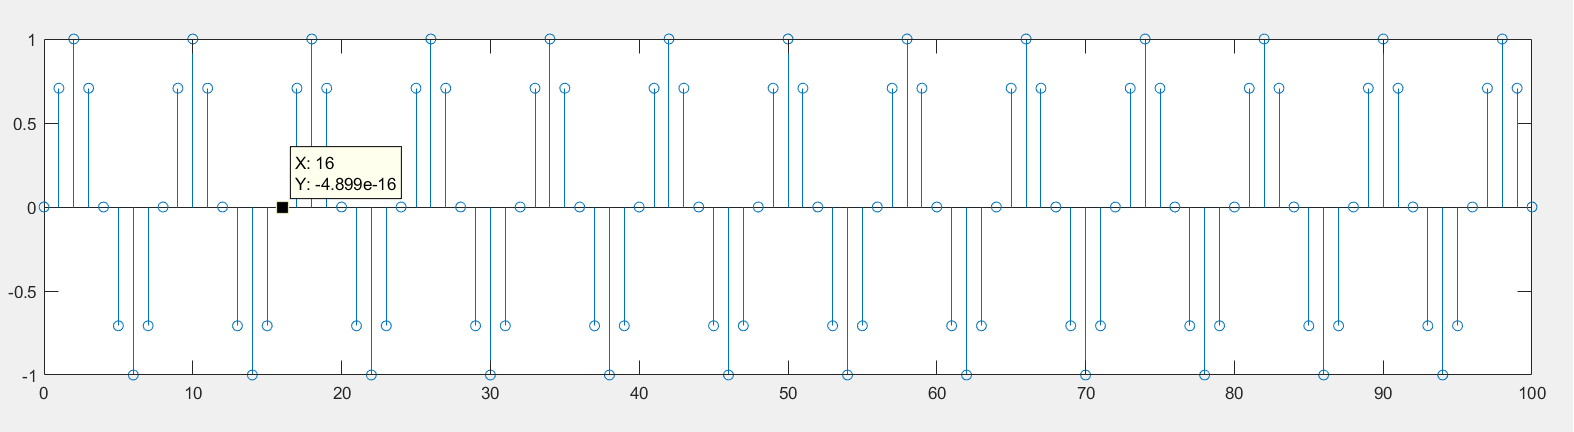
\includegraphics[width=15cm]{IMAGENES/T1_val1.png}
        \caption{Valor de la muestra 16 para y1.}
\end{figure}

\begin{figure}[h]
    \centering
        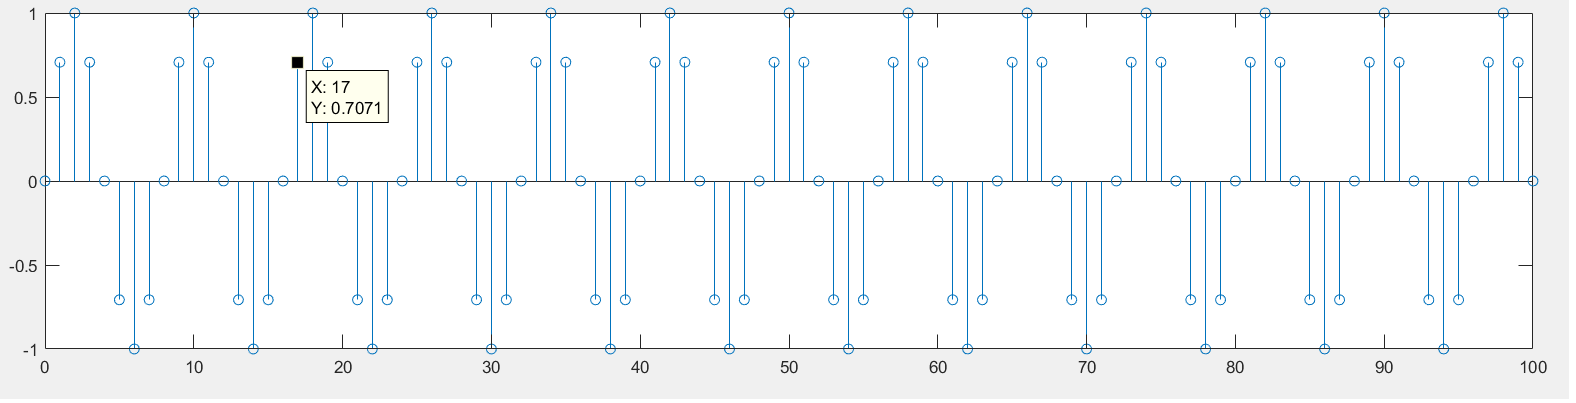
\includegraphics[width=15cm]{IMAGENES/T1_val2.png}
        \caption{Valor de la muestra 17 para y1.}
\end{figure}

\begin{figure}[h]
    \centering
        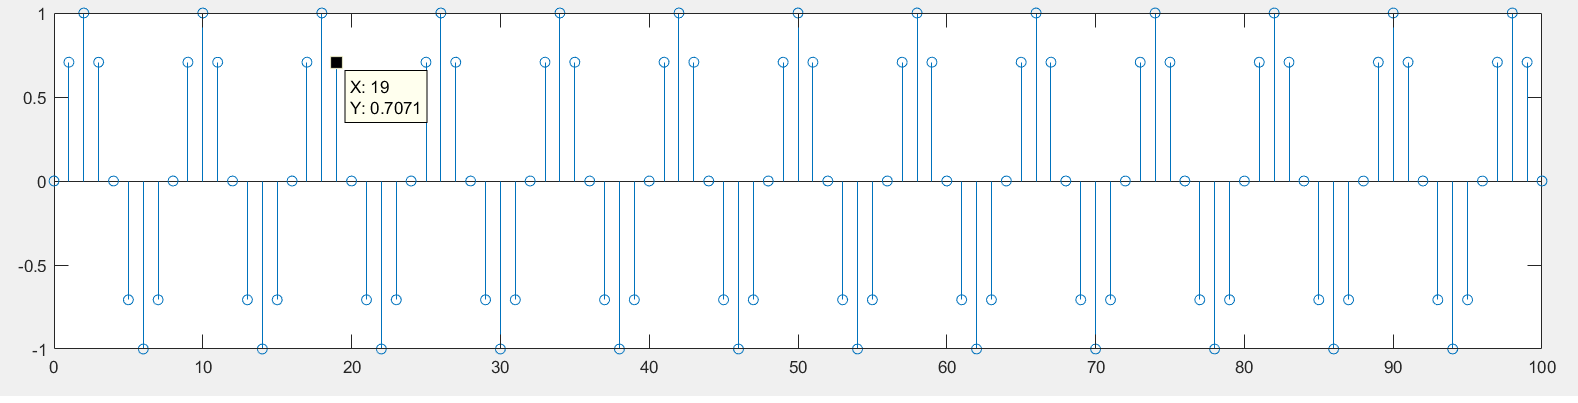
\includegraphics[width=15cm]{IMAGENES/T1_val3.png}
        \caption{Valor de la muestra 19 para y1.}
\end{figure}

\begin{figure}[h]
    \centering
        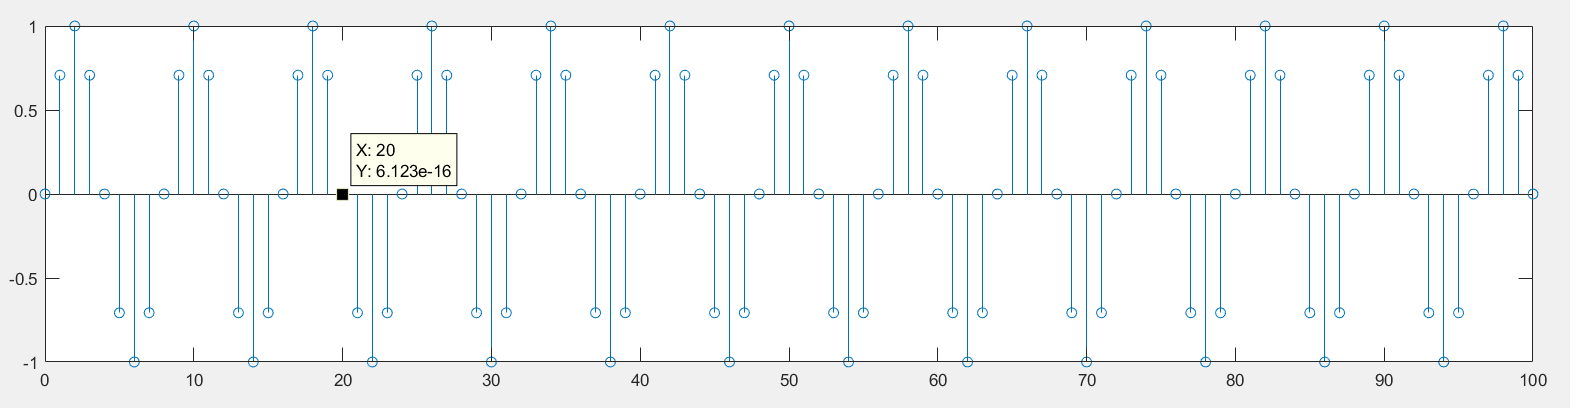
\includegraphics[width=15cm]{IMAGENES/T1_val4.png}
        \caption{Valor de la muestra 20 para y1.}
\end{figure}
\vspace{100mm}
\begin{figure}[h]
    \centering
        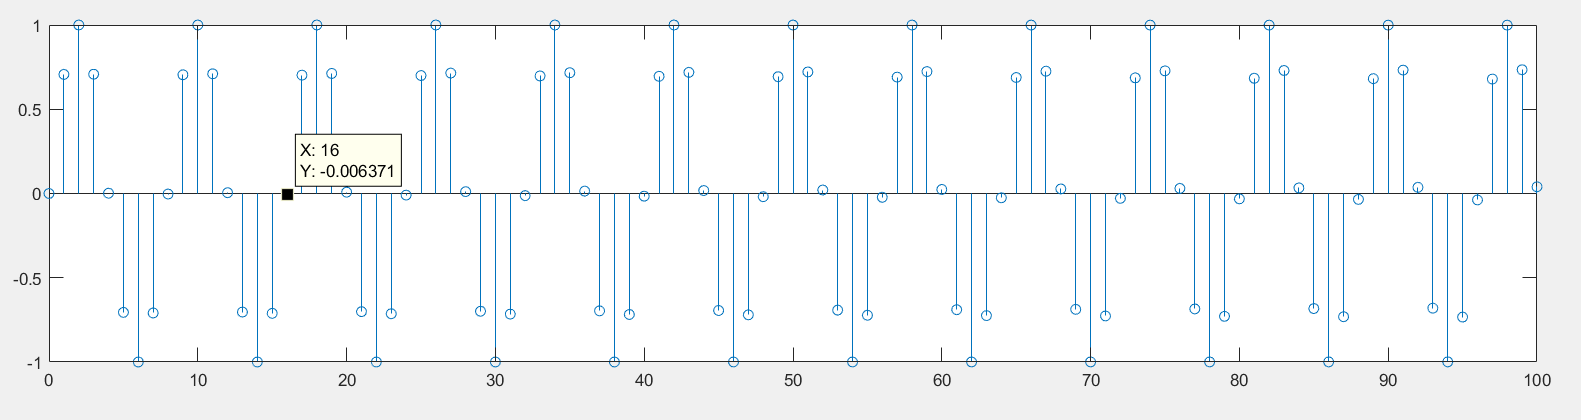
\includegraphics[width=15cm]{IMAGENES/T1_val5.png}
        \caption{Valor de la muestra 16 para y2.}
\end{figure}
\vspace{100mm}
\begin{figure}[h]
    \centering
        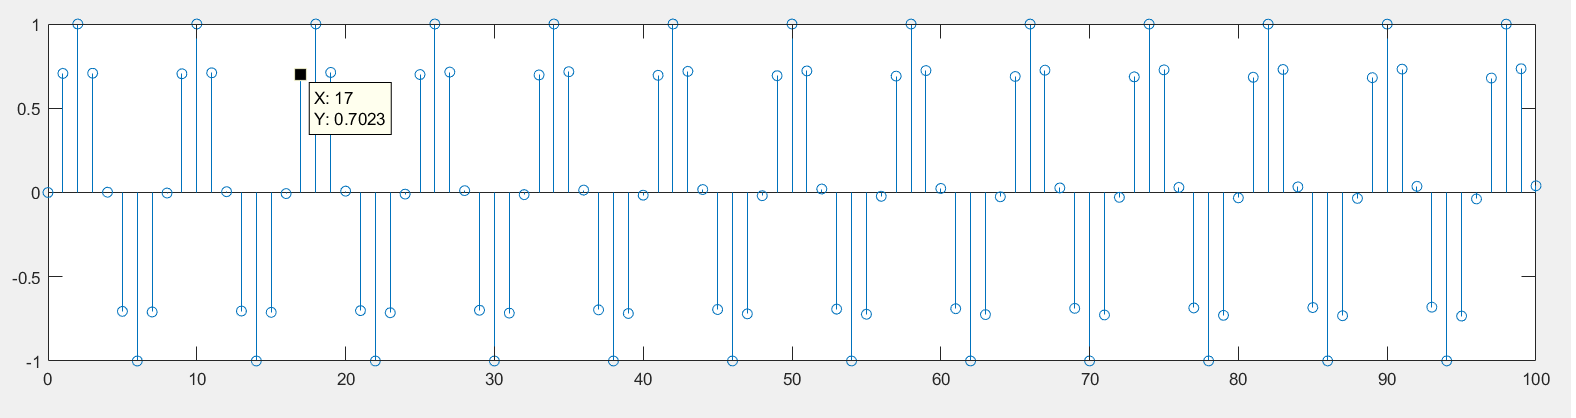
\includegraphics[width=15cm]{IMAGENES/T1_val6.png}
        \caption{Valor de la muestra 17 para y2.}
\end{figure}

\begin{figure}[h]
    \centering
        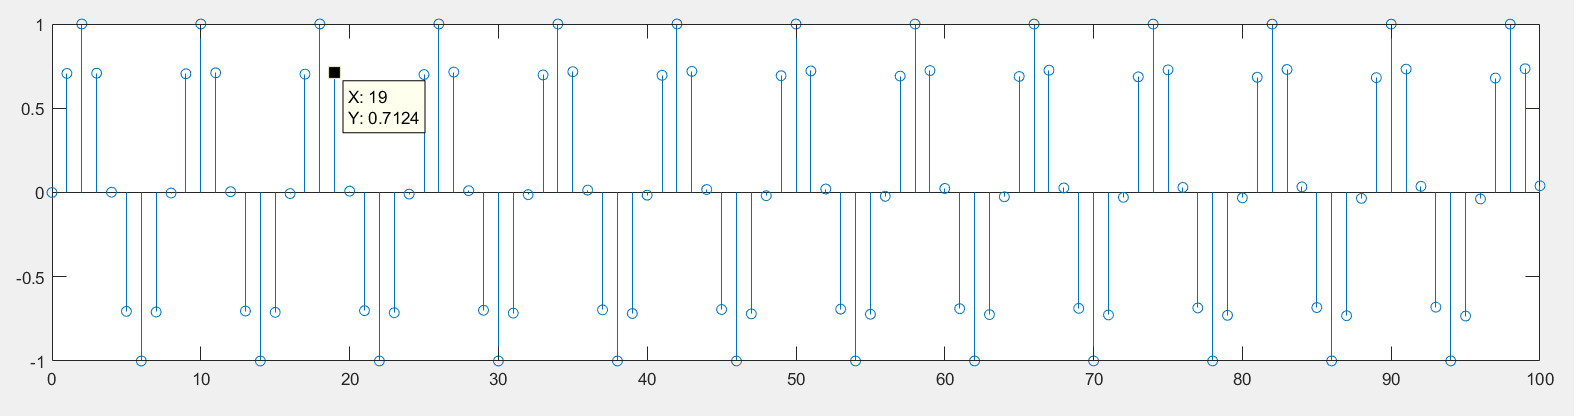
\includegraphics[width=15cm]{IMAGENES/T1_val7.png}
        \caption{Valor de la muestra 19 para y2.}
\end{figure}

\begin{figure}[h]
    \centering
        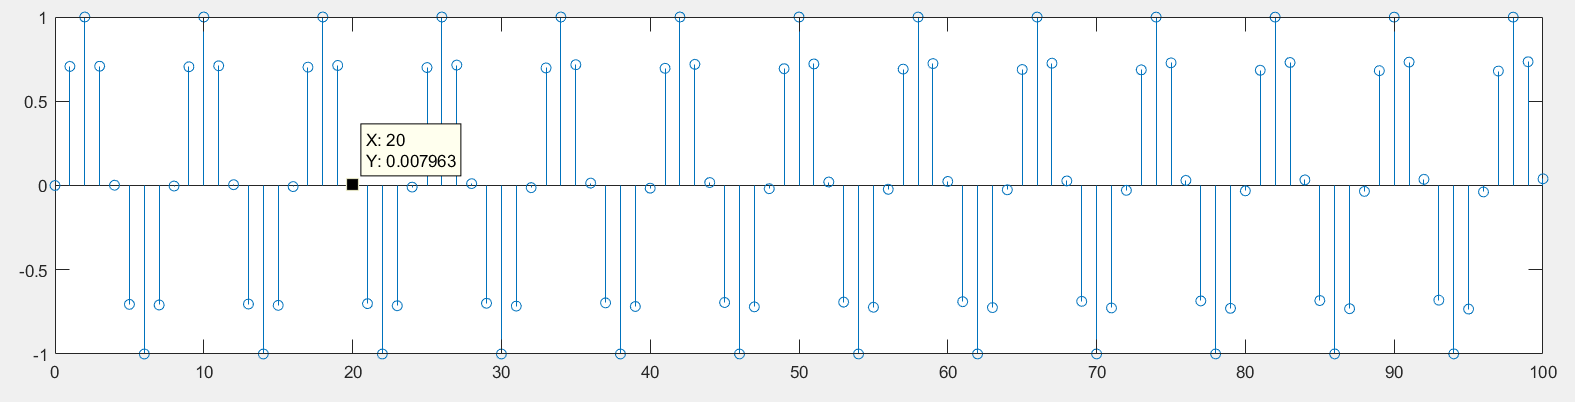
\includegraphics[width=15cm]{IMAGENES/T1_val8.png}
        \caption{Valor de la muestra 20 para y2.}
\end{figure}
\vspace{1mm}

\section{Resultados Observados}
Tenemos que una señal periódica se define como:
$$x(n+N)=x(n)$$
Donde $n$ es el número de muestras y es un entero. Entonces tenemos que una señal sinusoidal está definida como:
$$sin(wn+\theta)$$
Donde $w$ es la frecuencia en radianes por muestra y $\theta$ es la fase. Si la señal es sinusoidal-
periódica se tiene que cumplir la siguiente propiedad:
$$sin(wn+\theta)=sin(w(n+N)+\theta)$$
que nos conduce a deducir que:
$$2\pi k=wN$$
donde $k$ es un entero arbitrario. Si expresamos $w=2\pi f_0$ tenemos que:
$$f_0=\frac{k}{N}$$
Esto significa que la frecuencia en ciclos por muestra $f_0$ debe ser un número racional para que la sinusoidal sea periódica.
A la menor $N$ se le denomina frecuencia fundamental y representa cada cuántas muestras se repetirá la señal.\\\\
Para nuestro caso tenemos 2 señales sinusoidales con $f_0$ de valores:
$$f_A=\frac{1}{8}\frac{x_1}{\pi}$$
$$f_B=\frac{1}{8}\frac{x_2}{\pi}$$
Donde $x_1$ es el valor de $\pi$ más preciso y $x_2$ es el valor menos preciso. Para $x_1$ tenemos que la señal se repite cada 8 muestras, como se esperaría ya que $N=8$, y para $x_2$ tenemos que la muestra se repite cada 150 muestras, si es que se repite.
\\\\
Es observable que la diferencia entre los valores de las muestras en la figura 1 y 4 es muy pequeña, siendo poco estrictos se consideran cero por ser del orden de $1x10^{-16}$. Además, para la figura 2 y 3 se observa un valor congruente lo cual, juntando ambos fenómenos resulta en una señal periódica.
\\
Para el caso de la figura 5 y 8, si bien los valores también son pequeños, no lo son tanto comparado a sus homónimos mostrados en las figuras 1 y 4 respectivamente, por lo que ya son cifras que deben ser consideradas. Además, los valores de las figuras 6 y 7 aunque son cercanos, no son iguales, entonces no se puede considerar a esta función como periódica.

\section{Conclusiones}
Se consiguió observar la importancia de $\pi$ en el argumento de la función seno para demostrar la periodicidad de esta en tiempo discreto ya que, con un valor más exacto del valor $\pi$, se obtiene una señal que, despreciando cifras significativas, puede considerarse como periódica. 
\\
Caso contrario sucede para la segunda función. Cuando solo se utiliza un valor poco aproximado a $\pi$ ya que es notorio como esta variación, provoca cambios más significativos comparado con la primera función.

\section{Bibliografía}
\begin{thebibliography}{0}
  \bibitem{Libro3}Proakis J $\&$ Manolakis D.(2007).Tratamiento Digital de Señales. 4a Edición.PEARSON Pretince Hall 
\end{thebibliography}

\end{document}